\chapter{Exemplaric Implementation Using Game Engines as Renderers and Frontends}
\label{chap:implementations}
In this chapter the concept presented in \ref{chap:conceptual-design} will be implemented using a game engine as renderer and frontend. After a brief overview of the goals and constraints of this specific implementation, it will look into reasons why games engines are suited for implementing the concept and how one was chosen for this implementation. Analogue to the steps described in the concept, this chapter will show how an existing environment was reconstructed to be used as a scene and how a robot was imported into this scene and optimized to work in the game engine. Further, it will show how mutators were implemented and used in the scene and compare different approaches to identifying objects. Lastly, this chapter shows how records were saved and how this implementation performed during recording sessions.

%////////////////////////////////////////////////
\section{Goals and Constraints of the Implementation}
\label{section:goals-and-constraints}
Inspired by a thesis written by Schweitzer in 2017 that approached using \acsp{CNN} that detect doors on autonomous robots \cite{Schweitzer2017}, the goal of this thesis' implementation became to generate records that could be used to train \acsp{CNN} that detect doors.\\ 
The environment chosen for this implementation was the second floor of building "A" of University of Applied Sciences Mannheim as this building houses the Faculty of Computer Science and the Institute of Robotics is located in the second floor.\\
This implementation of the concept had the working title \emph{\ac{VERE}}. While it produced records that could be used to train \acsp{CNN}, no such tests were performed due to time-constraints.

\section{Using Game Engines}
The decision to use game engines to implement the concept was based on the observation that video games have always striven after improved visual presentation and more intuitive user interaction in order to attract customers, leading to the general availability of game engines that feature impressive graphical detail (as demonstrated in figure \ref{fig:unity-demo-graphics}), intuitive methods to interact with users and great performance on modern computer systems. Their ability to produce realistic images in real-time made them an attractive alternative to traditional offline renderers.
\begin{center}
\noindent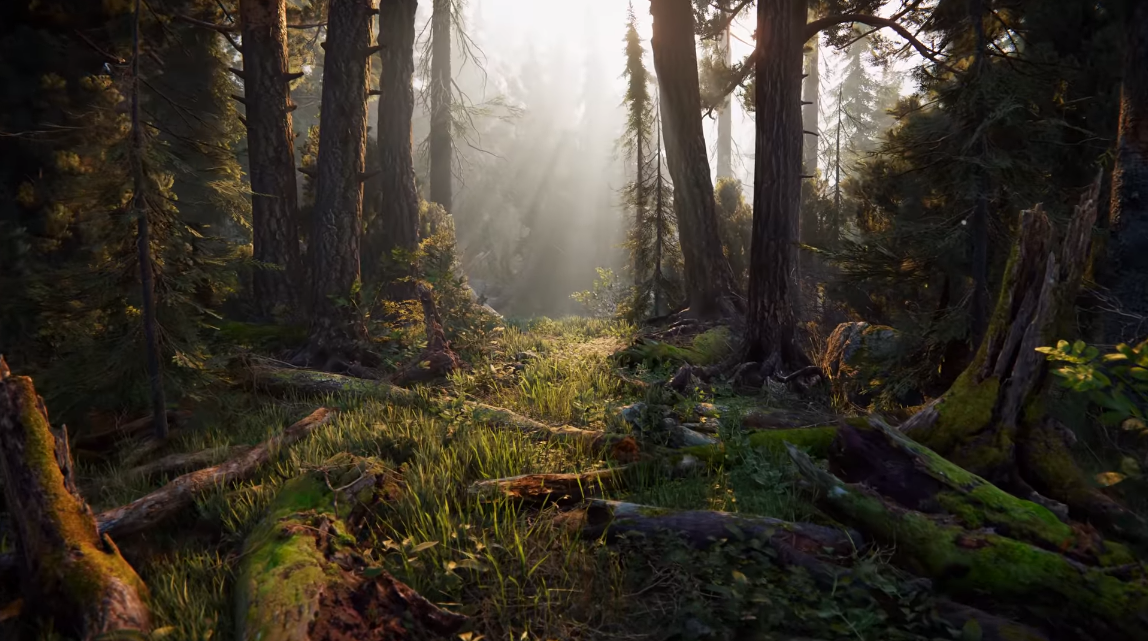
\includegraphics[width=14cm]{tex/img/ch05/UnityGraphicsDemo.png}
\captionof{figure}[Unity Engine demo]{Unity Technology's "Book of the Dead" promotional video \cite{UnityDemoRealtimeTeaser}}
\label{fig:unity-demo-graphics}
\end{center}

New rendering-technologies that improve the quality of rendered images and performance of the rendering-process are being developed and published by both proprietary and open-source developers. A current example of a new technology recently published is NVIDIA's proprietary "RTX"-technology \cite{NVIDIARTX} that features "Hybrid Rasterization and Ray Tracing" \cite{NVIDIARayTracing} to combine raytracing and conventional rasterization in the rendering-process. A public demonstration of this new technique was shown running on the "Unreal Engine" in a short video (figure \ref{fig:unreal-demo-graphics})\cite{UnrealDemoReflections}.
\begin{center}
\noindent
\includegraphics[width=14cm]{tex/img/ch05/UnrealGraphicsDemo.png}
\captionof{figure}[NVIDIA RTX demo]{Demonstration of NVIDIA RTX and Microsoft DXR running on the Unreal Engine \cite{UnrealDemoReflections}}
\label{fig:unreal-demo-graphics}
\end{center}

%////////////////////////////////////////////////
\subsection{Choosing a Game Engine}
The decision which game engine to use to implement the concept was based on a set of factors (inspired by criteria defined by Cowan \textit{et al} \cite{6901570}) that needed to be considered:
\begin{description}
\item [Stability] While the goal of using game engines as real-time renderers is to generate records quickly, recording sessions may take several hours. The software needs to maintain stable operation because recording sessions may run un-supervised and crashes may be detected only hours later.
\item [Crossplatform] Support of multiple platforms serves multiple purposes. First it aims to avoid platform-specific problems that may either be already existent or yet to come. Operating-system updates can cause software to malfunction as was recently seen with multiple updates of the Windows operating system \cite{heiseWindowsUpdate}. Secondly, supporting multiple platforms greatly extends the potential groups of users. Users that own licenses for proprietary operating systems will be able to run the software on their current systems while users that lack licenses to proprietary operating systems may chose a free operating system. The third and very important aspect of crossplatform-capabilities is that developers only need to implement code specific to a game but no code specific to platforms. This allows to compile a game for multiple platforms without spending any time on the target platforms' specifics.
\item [Features] As this thesis' concept aims to generate labelled images of excellent quality, the game engine used for rendering said images must feature rendering capabilities that produce realistic output. This requires extensive support of post-processing features like ambient occlusion, anti-aliasing, depth-of-field and other shading-techniques.
\item [Maintenance] Software is expected to be operable for a certain period. While games may run on modern systems for few years, programs used in sophisticated fields of use like research aim to be used and developed further for many years. Programming those comes at considerable development cost which is why one important factor is the expected time a game engine enables software to run on modern systems. One way to evaluate this factor is to study when a game engine was first publicly announced, what games are being published that use the engine and in what intervals it is updated. Dependencies introduced by game engines further add to potential problems with software becoming outdated and unable to use on modern systems. 
\item [Licensing] Like most other software, game engines are usually distributed with licenses that specify under what conditions and for which purposes they may be used. Many engines that power popular games today are exclusive to their developer studios or publishers and are not available for public use (e.g. \emph{EA DICE}'s exclusive \emph{Frostbite} that powers the \emph{Battlefield} game-series or \emph{id Software LLC}'s exclusive \emph{id Tech 6} which \emph{Doom (2016)} was based on). Contrary to those, some modern proprietary game engines may be used for free for educational or private use (such as the CryEngine, Unity Engine and Unreal Engine).
\item [Community] When it comes to become acquainted with working with game engine, an active community of developers can prove very useful as documentation may become obsolete when update-cycles of game engines are very short. Open-source projects allow developers to use and learn from others' code so one may be more likely to find open-source projects for popular game engines than less popular ones.
\item [Assets] Some developers of game engines (such as Unity and Unreal Engine) offer access to free or paid assets (such as 3D models, sound and even code) that can be used in projects. Using existing assets saves time during development.
\item [Tools] Popular game engines are usually distributed with alongside with tools that streamline the development of games. Some come with feature-rich all-in-one software suites (e.g. Unity, CryEngine and Unreal Engine) that cover tasks like world-building, scripting and compiling. Others provide separate tools like world-editors, conversion-tools (to convert files to proprietary formats) or compilers (e.g. Source Engine).
\end{description}

After evaluating modern and popular game engines considering the abovementioned criteria (as shown in \ref{table:game-engines}), the Unity game engine was used for implementation of the concept of this thesis. It was chosen because of its crossplatform-capabilities \cite{UnityPlatformSupport}, regular updates (between two and four updates a month in 2018 \cite{UnityDownloadArchive}), free use for educational purposes \cite{UnityForEducation}, active community of developers \cite{UnityForum} and built-in editor-application. It features a free post-processing stack \cite{UnityPostProcessingStack} and built-in editor (shown in figure \ref{fig:unity-editor}) that allows developers to build scenes, configure objects in scenes and test their games.
\begin{center}
\noindent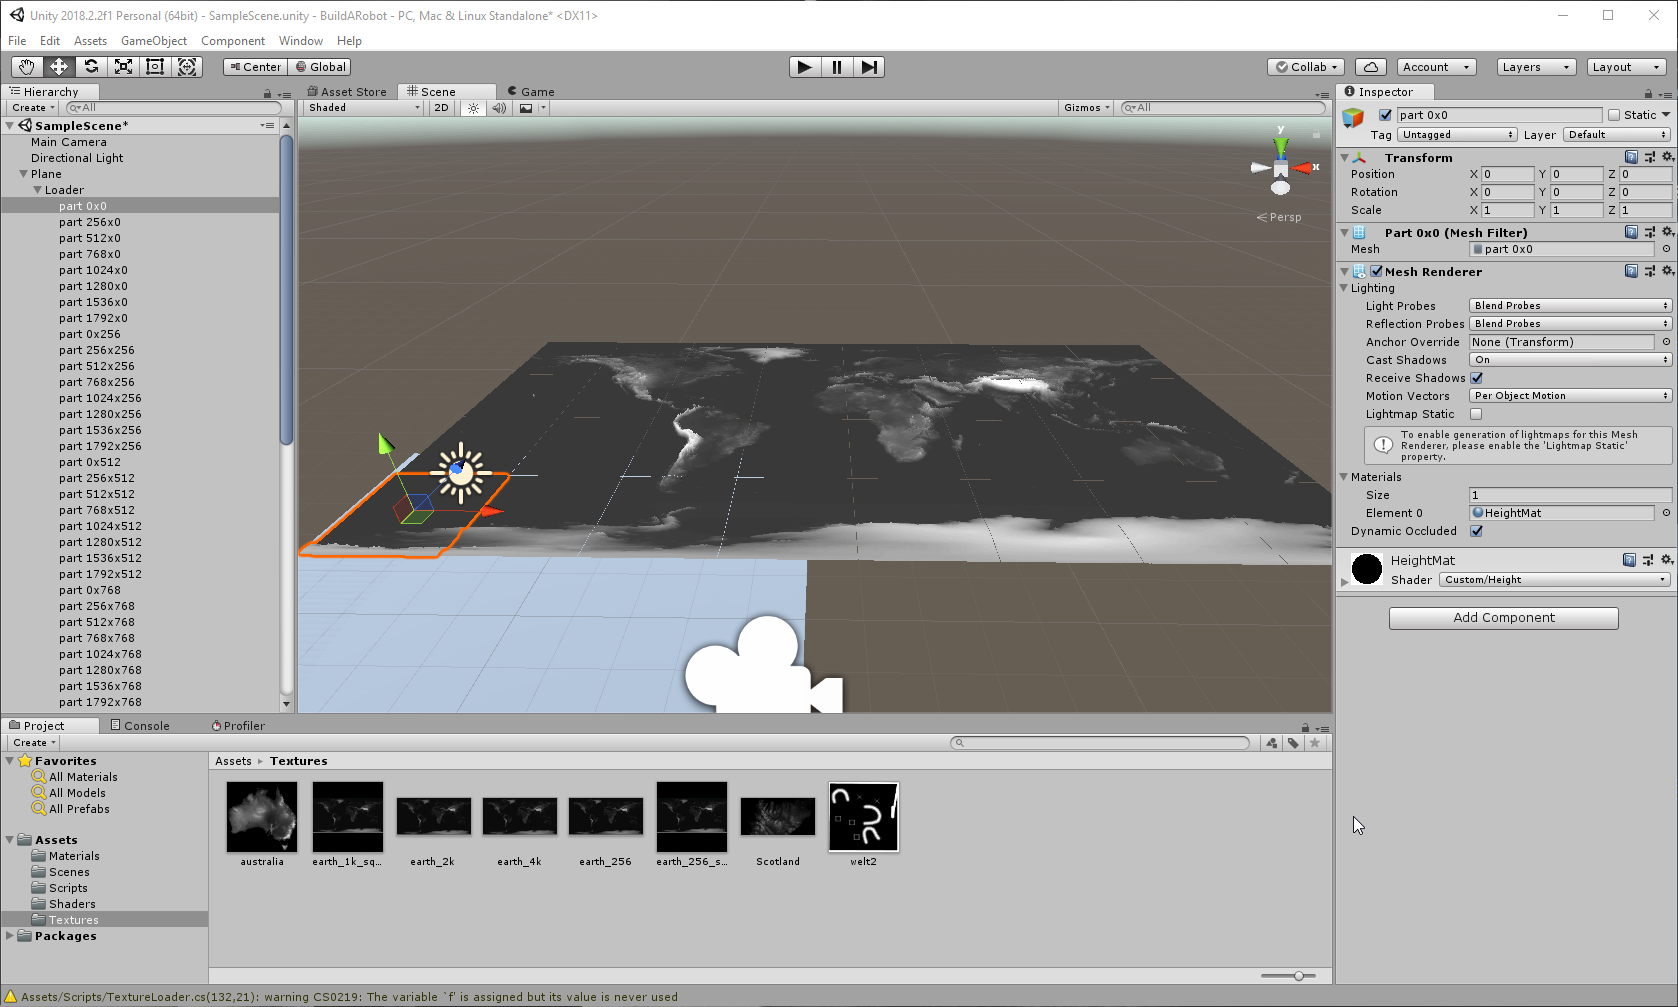
\includegraphics[width=14cm]{tex/img/ch05/UnityScreenshot.png}
\captionof{figure}{The Unity Editor}
\label{fig:unity-editor}
\end{center}

%////////////////////////////////////////////////
\section{Designer: Building the Scene}
\subsection{Rebuilding a real environment}
As stated in \ref{section:goals-and-constraints} the environment used to base the scene on was the second floor of building "A" of University of Applied Sciences Mannheim. However at this time no 3D model of the floor, let alone the building existed so it had to be handcrafted using the resources that were available: a floor plan (shown in Figure \ref{fig:floor-plan-image}) and measurements taken by hand.

\begin{figure}[htp]
    % preliminary
    \sbox\twosubbox{%
      \resizebox{\dimexpr.9\textwidth-1em}{!}{%
        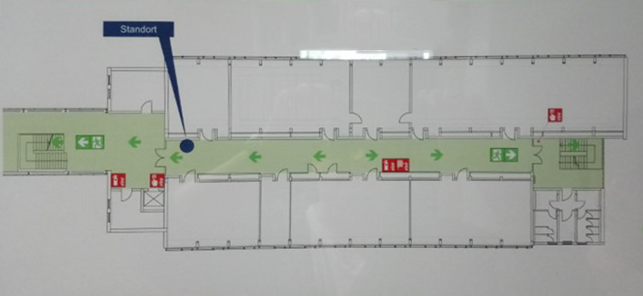
\includegraphics[height=3cm]{tex/img/ch05/FloorPlan03_small.JPG}%
        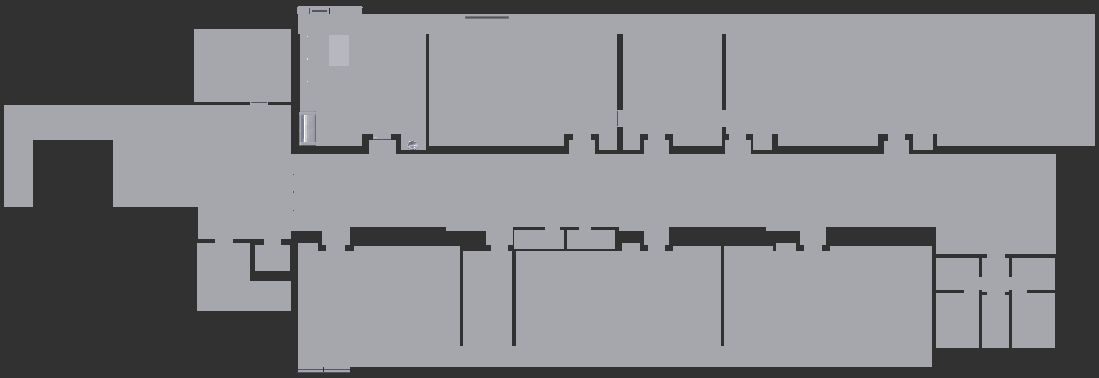
\includegraphics[height=3cm]{tex/img/ch05/BlenderFloor01.png}%
      }%
    }
    \setlength{\twosubht}{\ht\twosubbox}
    % typeset
    \centering
    \subcaptionbox{\label{fig:floor-plan-image}}{%
      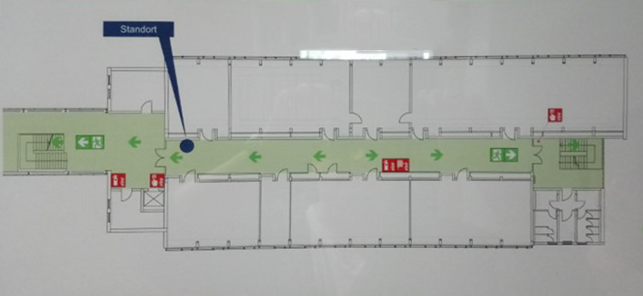
\includegraphics[height=\twosubht]{tex/img/ch05/FloorPlan03_small.JPG}%
    }\quad
    \subcaptionbox{\label{fig:floor-plan-blender}}{%
      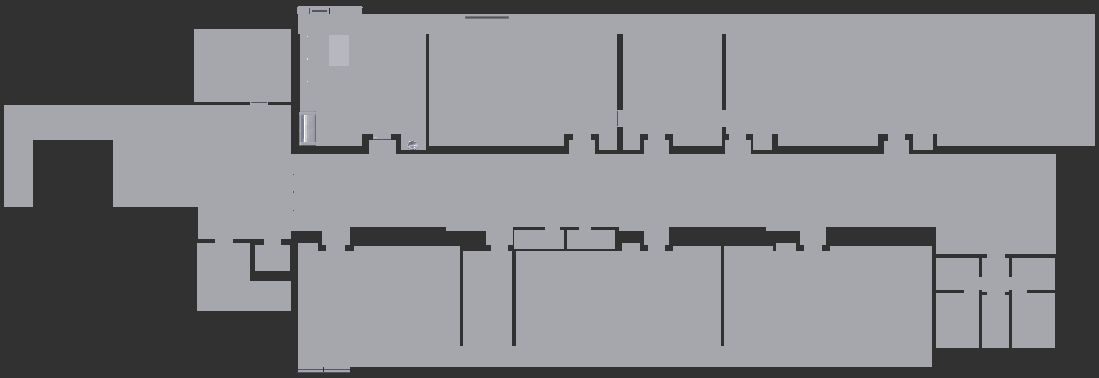
\includegraphics[height=\twosubht]{tex/img/ch05/BlenderFloor01.png}%
    }
    \caption{Floor plan, photo (\ref{fig:floor-plan-image}) and reconstruction in Blender (\ref{fig:floor-plan-blender})}
\end{figure}

Figure \ref{fig:floor-plan-blender} shows the reconstruction of the basic layout of the floor in the 3D modeling software Blender. As the goal of this implementation was to generate records used for detecting doors, special attention had to be paid to modeling the doors in this floor. This required taking measures of the doors themselves, their handles and frames as well as reconstruction of the properties of their surfaces. Figure \ref{fig:doors} shows the various doors present on this floor: office doors (shown in \ref{fig:door01} featured metallic handles, a black and matte metal surface and were broader than most other doors. Doors to lecture rooms (\ref{fig:door02}) had blue matte metal surfaces and were not on the same level as the walls but inset into the walls. They also had glass-panels located right above them. The portals (\ref{fig:door03}) to the hallway that lead to the lecture rooms, one present at each end of the hallway, had glass doors and panels and matte black metal beams and frames. Lastly there were doors to storage rooms (\ref{fig:door04}) that did not feature great geometrical detail as the other doors did. They blended into the wall and featured knobs and hinges that were noticeably shiny.

\begin{figure}[htp]
    \sbox\twosubbox{%
      \resizebox{12cm}{!}{%
        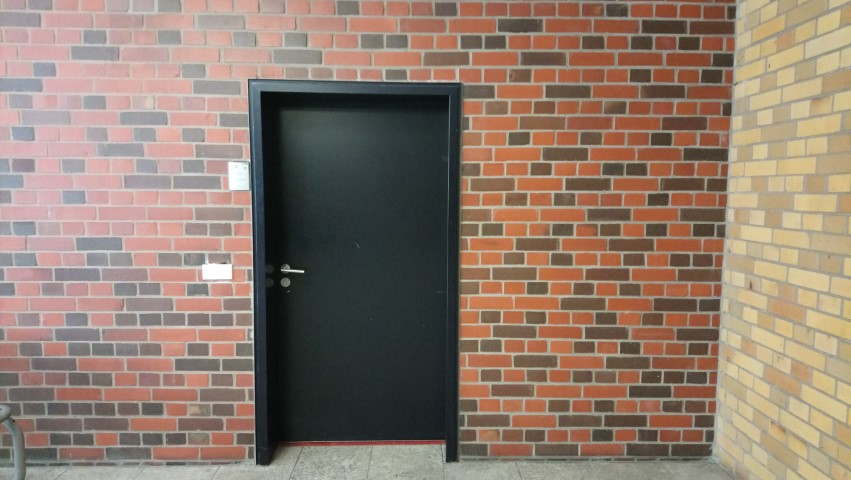
\includegraphics[height=6cm]{tex/img/ch05/Door01_small.JPG}%
        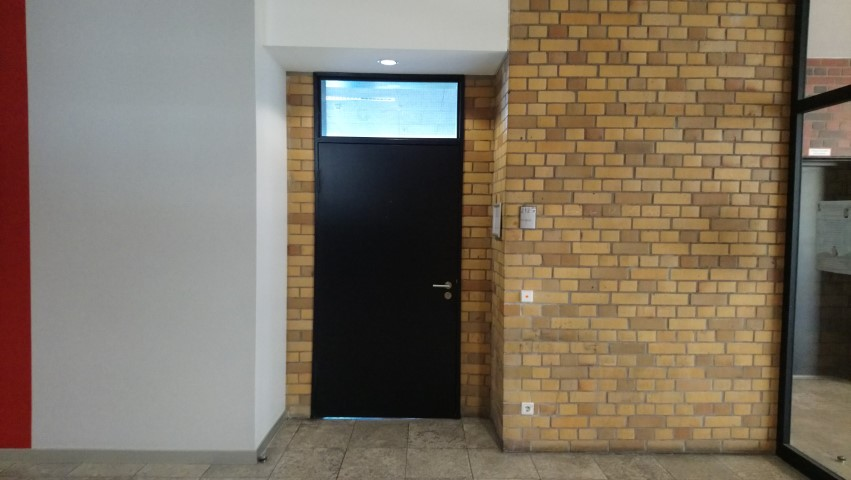
\includegraphics[height=6cm]{tex/img/ch05/Door02_small.JPG}%
      }%
    }
    \setlength{\twosubht}{\ht\twosubbox}
    \centering
    \subcaptionbox{\label{fig:door01}}{%
      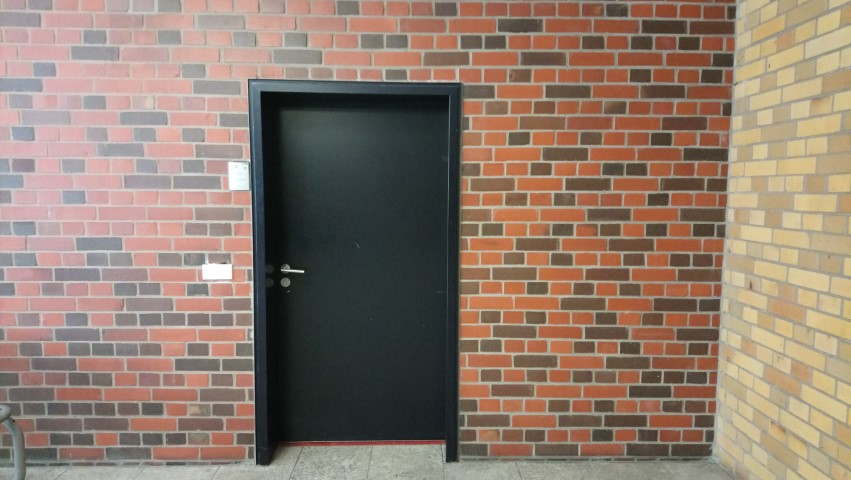
\includegraphics[height=\twosubht]{tex/img/ch05/Door01_small.JPG}%
    }\quad
    \subcaptionbox{\label{fig:door02}}{%
      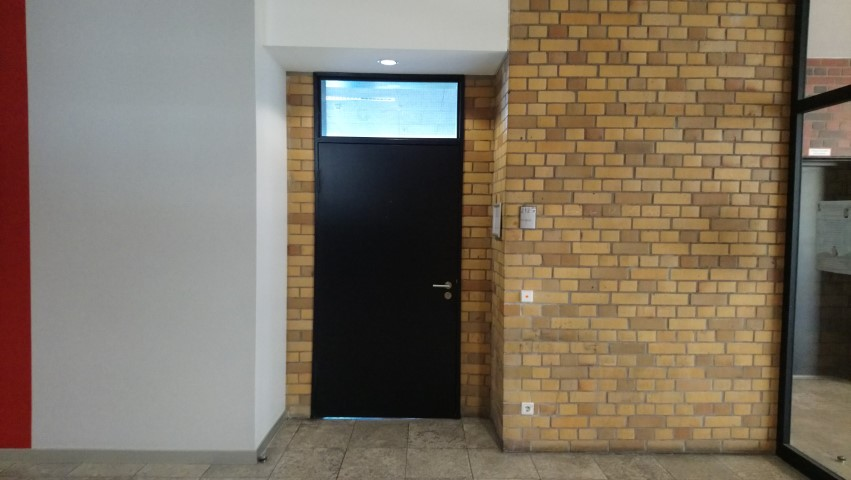
\includegraphics[height=\twosubht]{tex/img/ch05/Door02_small.JPG}%
    }\\%quad
    \subcaptionbox{\label{fig:door03}}{%
      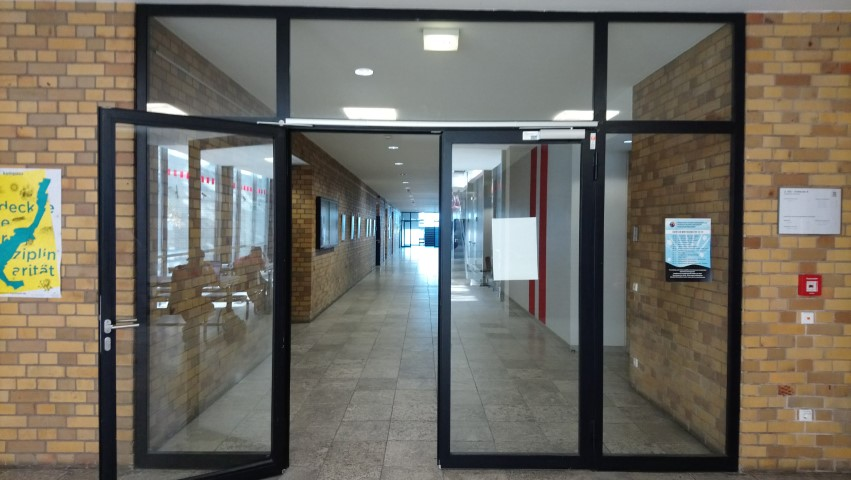
\includegraphics[height=\twosubht]{tex/img/ch05/Door04_small.JPG}%
    }\quad
    \subcaptionbox{\label{fig:door04}}{%
      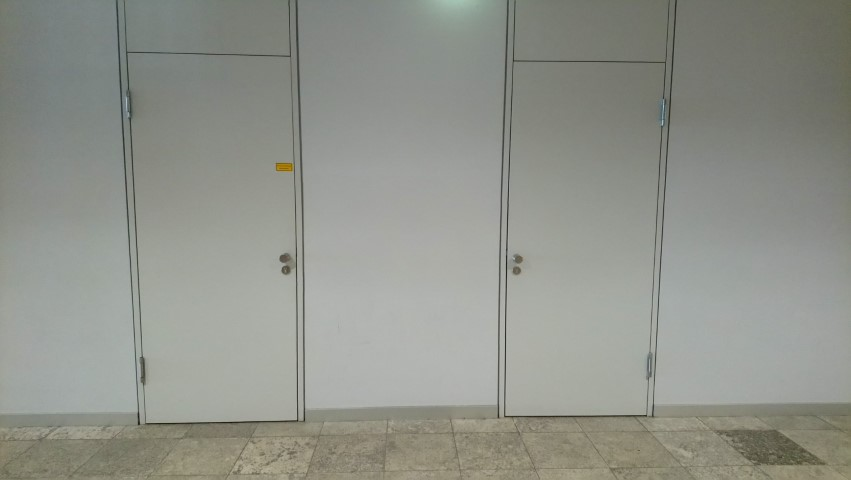
\includegraphics[height=\twosubht]{tex/img/ch05/Door05_small.JPG}%
    }
    \caption{Various different doors on the floor}
    \label{fig:doors}
\end{figure}

The reconstructed doors could now be used to render very detailed door meshes with realistic surfaces. However other objects also had to be reconstructed: as lighting would have great influence on generated images, large window facades that cover the building's exterior and feature blinds were added to the scene. A set of other common objects present in the floor like lamps and air-conditioning pipes on the ceiling, radiators and tables were also reconstructed.\\
Figure \ref{fig:unity-scene-a205} shows the final reconstruction of room \emph{"A205"} which is the first room on the second floor of the building. It features windows with blinds that cast shadows on the walls and objects and it features obstacles (such as tables) that may occlude other objects of interest such as the blue door. The reconstructed room does not feature any chairs, even though there were chairs present in the real room. They were left out to enable robots to navigate through the room easily without having to take care of maneuvering in tight spaces between chairs. However chairs would have contributed to making the room appear more realistic as chairs may have occluded objects of interest and added to the complexity and variety of the scene overall.

\begin{figure}[t]
    \centering
    %\noindent
    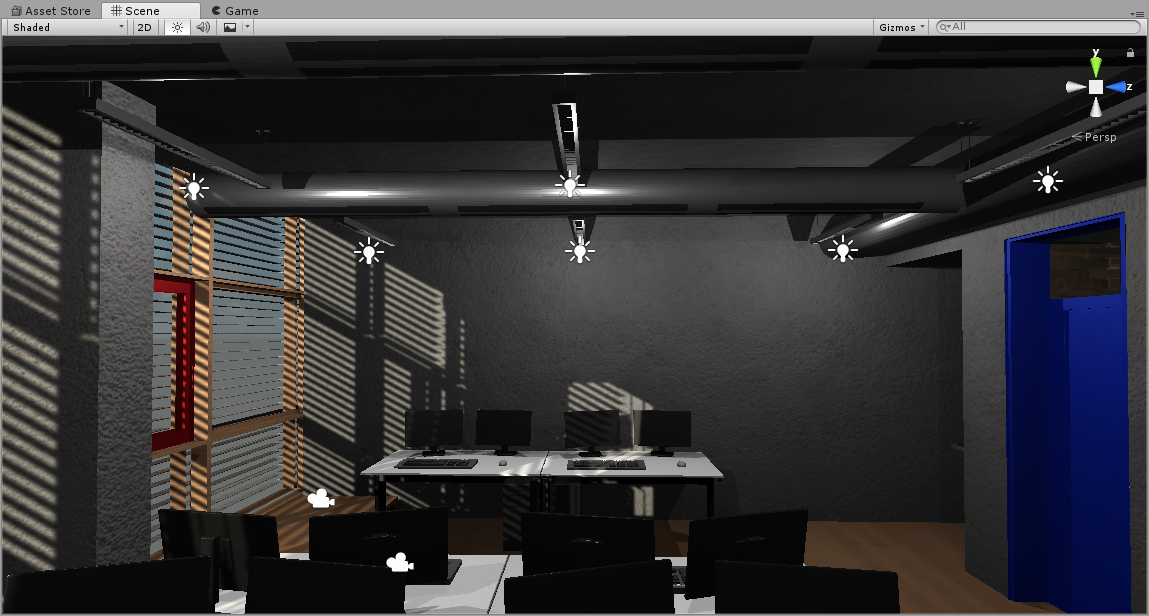
\includegraphics[width=12cm]{tex/img/ch05/UnitySceneA205_02.png}
    \captionof{figure}{Reconstruction of room A205 in Unity Editor}
    \label{fig:unity-scene-a205}
\end{figure}

%////////////////////////////////////////////////
\subsection{Adding Robots to the Scene}
\subsubsection{Importing Robots}
Once the scene is set up, a robot is needed for \acs{AI} engineers to navigate around the scene and capture records. For this implementation the robot model "Pioneer 3AT" was chosen as the Institute of Robotics of University of Applied Sciences Mannheim works with "Pioneer"-robots and there were \ac{URDF} files of it available \cite{AmrRosConfig} online.\\
There were few libraries that provide methods to import robots using URDF-files into Unity, an extensive one was \emph{"ROS\#"} which was developed by Siemens AG. Siemens described it to be \textit{"a set of open source software libraries and tools in C\# for communicating with ROS from .NET applications, in particular Unity3D"} \cite{RosSharp}. This project implemented connecting to ROS instances, ROS' publish/subscribe pattern and importing robots into Unity scenes, however its software design introduced some potential problems: 
\begin{enumerate}
    \item Importing robots using URDF-files was done by downloading URDF-files from running ROS-instances. The need for a running ROS-instance would add to \ac{VERE}'s system requirements.
    %ros-sharp/Unity3D/Assets/RosSharp/Scripts/Urdf/Editor/UrdfComponents/UrdfRobotExtensions.cs
    \item ROS\#'s URDF importing component required the URDF files to be present in the "Asset" folder of Unity projects. This meant that URDF files downloaded from remote locations needed to be written to disk and compressed archives that contained additional files like meshes and textures needed to be extracted to disk first.
    \item Even though robots imported by ROS\# had correct hierarchy of body parts and correct physical properties (as defined in the robots' URDF), Unity's physics engine often times failed to simulate physics at run-time, leading to robots being unable to move, falling through floors or being propelled into the air.
\end{enumerate}
To solve these problems, a library for parsing URDF-files, \emph{"URDFParser.NET"}, was implemented. The first two problems were solved by implementing a set of interfaces that represent filesystems, directories and files (\ref{fig:filesystem}) for local filesystems and ZIP-archives (using the open-source library \emph{"DotNetZip"} \cite{DotNetZip}) as URDF-files including meshes and textures were usually distributed as ZIP-archives. These interfaces could also be implemented to read files from remote locations such as FTP-servers or websites for future scenarios and use-cases.
\begin{center}
\noindent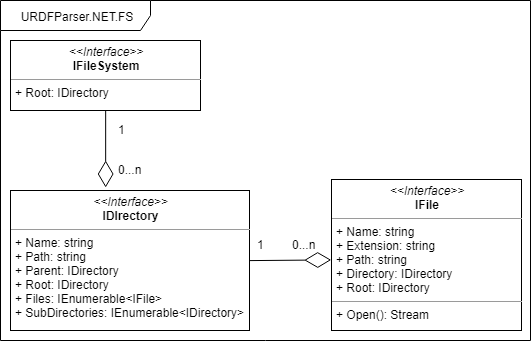
\includegraphics[width=14cm]{tex/img/ch05/URDFParser_FileSystemInterfaces04.png}
\captionof{figure}{Interfaces for filesystems, directories and files}
\label{fig:filesystem}
\end{center}
Contrary to ROS\#'s approach of interpreting hard-coded XML-elements, in URDFParser.NET parsing the URDF-files was implemented by defining \acp{DTO} for the different URDF-elements. URDF-Files could then be deserialized using these \acsp{DTO} with the \emph{"XmlSerializer"}-class provided by the .NET-Framework \cite{XmlSerializer}.\\
The third problem with ROS\#'s implementation, faulty behaviour of physical bodies (also called \emph{"rigid bodies"} in the Unity Engine), required manual adjustments to the imported robot models: rearranging the robots' hierarchy so at all times a physical object may have only one physical child object solved robots' inability to move. Ensuring that colliders of physical parts (such as wheels and chassis) did not intersect with each other eliminated the problem of robots spontaneously launching into the air. 

\subsubsection{Controlling Robots}
Robots imported into Unity needed to be controllable by \ac{AI} engineers. This could be done in different ways. with some of those depending on the type of drive a specific robot featured:
\begin{description}
    \item [Wheel Drives] Robots may feature wheel-joints that can rotate on their local $x$ and $y$ axis. Rotating a wheel's $y$ axis allows to use it for steering while applying torque to its $x$ axis would move it and its connected bodies across surfaces, just like real-world wheels work. This technique can be used for most wheeled robots by limiting rotation of the $y$ axis to wheels that should not steer (e.g. the rear wheels of motor cycles).
    \item [Connected Limbs] Limbs of robots can be connected using hinge joints that allow rotating connected bodies along one or more axis. Most industrialized robots feature three or more controllable axis and could be implemented in Unity by connecting two limbs via one hinge-joint each, allowing movement in one axis. Industrialized robots operate from a fixed position in 3D space.
    \item [Legged Movement] Extending on the techniques used for implementing industrialized robots, one can combine multiple limbs to a body and move these limbs via hinge joints to simulate legged robots. The major difference from industrialized robots is that legged robots do not reside in a fixed position but move their bodies in 3D space.
\end{description}
While simulating wheel drives, connected limbs and legged movement is possible in Unity Engine and other engines, they come at the cost of complex configuration and intensive testing. An alternative to physical simulation is by simply fabricating the illusion of such, presuming that the scenario at hand does not require exact simulation of movement but allows for fabricated approximations:
\begin{itemize}
    \item Wheel drives can be reconstructed by wheel joints that allow for rotation in the $x$ and $y$ axis, however they do not require force directly applied to them for rotation . Applying directed force at a robot's body for acceleration and deceleration and applying torque force for turning would indirectly affect the wheels and thus fabricate the illusion of real wheel drives. 
    \item Connected limbs can be imitated by creating a parent-child hierarchy for each connected limb. Making use of Unity's transforms, child limbs of parent limbs will directly be affected by any change to the parent's transform: for instance, rotating the base limb of a robot arm would also effectively move all of its child limbs with it.
    \item Legged movement would be the hardest do fabricate in a way that behaves realistic. Most game engines feature animation systems that allows for replaying, looping and blending animations of complex body parts, resulting in movement that looks realistic. However it would not necessarily behave realistically as individual legs colliding with obstacles could lead to the whole body being moved, ignoring the friction of the other legs of a robot that may have contact to a surface and thus restrict movement of the robot's body.
\end{itemize}

Figure \ref{fig:pioneer3at} shows a "Pioneer 3AT" robot imported into Unity. The green cylinders represent the colliders of its wheels and it lacks any other colliders. Its only rigid body that had any mass and was simulated for gravity was its chassis. This combination of a single rigid body and one cylindrical collider for each wheel enabled the robot to appear and behave close to a real robot in the scene as neither collision with its chassis nor mass of its wheels were necessary for maneuvering it in the scene. Its wheels would turn when force is applied to its rigid body.

\begin{center}
    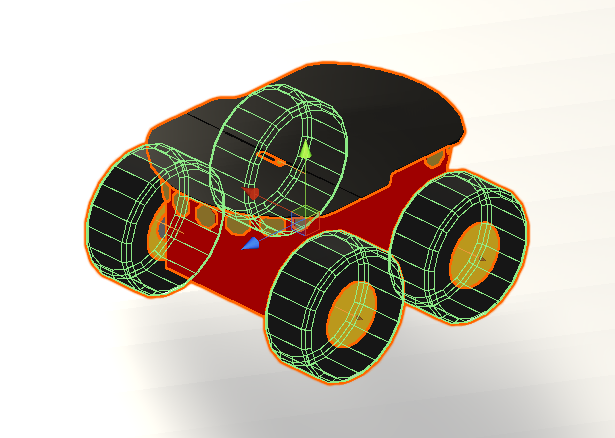
\includegraphics[width=0.39\textwidth]{tex/img/ch05/Pioneer3AT.png}
    \captionof{figure}{A "Pioneer 3AT" robot imported into Unity}
    \label{fig:pioneer3at}
\end{center}

Unity unifies input of various different input devices by providing an extendable set of values that either buttons and axis of one or multiple input devices can be mapped to. In its default configuration, Unity maps input for movement from both digital inputs like keyboards and analog inputs like joysticks to two axis, one for horizontal and one for vertical movement. As a result, pressing the "A" or "Arrow Up" buttons on a keyboard and pushing a joystick into the positive direction of its $y$ axis would affect the vertical input axis. In scripts, this could then be accessed by a simple call to $Input.GetAxis("vertical")$ which would return a value in the interval $[-1, 1]$ where positive values indicated a movement forwards and negative values indicated a movement backwards. Analogue to this, negative values of the horizontal axis would indicate movement to the left and positive values would indicate movement to the right.\\
In \ac{VERE}, the vertical axis for forwards and backwards movement was used to apply either a positive or negative force to the robot's body in its forward direction which would make it accelerate and decelerate. The horizontal axis was used to apply a torque force to its body, allowing it to steer. Due to the mass of the robot the applied torque force was not sufficient to move it while it was standing still, however it was strong enough to apply slight steering to the robot while it was driving, which in turn appeared realistic.

%////////////////////////////////////////////////
\section{Implementing Mutators}
The concept of this thesis proposed generating sets of diverse images by utilizing mutators to alter the appearance of single entities or whole scenes. Mutators would operate on a step-by-step basis, altering the state of an entity by each step. In this implementation, mutators would implement a simple interface \emph{IMutator} that provided methods to advance and reset itself. Three implementations of this interface were used to simplify the use of this interface for various applications: 
\begin{description}
\item [RangeMutator] Most attributes that were to be altered had numerical values that had to be incremented or decremented each step. \emph{RangeMutators} would have a \textit{FloatRange} associated to them that defined a value-range and step-size. These mutators could perform mutations on a single attribute of a single object using a value within the specified range of values and incremented or decremented this value using the specified step-size. RangeMutators would be used to manipulate most numeric values like light-intensity, the angles that doors were opened by and the orientation of the sun. The number of steps $s$ needed to complete one cycle of this mutator is $|\frac{maximum-minimum}{stepSize}|$ where $maximum$, $minimum$ and $stepSize$ are specified by a RangeMutator's FloatRange.
\item [MultiMutator] A single entity could hold many mutators and in order to group them and make them easily accessible to the MutationManager, those mutators would be added to and effectively encapsulated by \emph{MultiMutators}. Those would advance mutators in a serial fashion: it advanced the first child-mutator until the cycle of this child-mutator was completed. Then it would advance the second child-mutator by one step, reset the first one and continue advancing the first child-mutator again. The number of steps a MultiMutator needed to complete a cycle was directly dependent on the mutators it grouped. Given the set of its mutators $m$ a MultiMutator needed $\prod_{i=1}^{|m|} S(m_i)$ steps to complete a cycle, where $S(x)$ returns the number of steps a mutator $x$ needed to complete a cycle.
\item [ParallelMutator] There were cases where single mutators did not have great influence on scenes or did not have to have a whole mutation-step in a scene dedicated to them. For instance in this implementation, lamps in room A205 were mutated in parallel by using a ParallelMutator. These mutators would group other mutators like MultiMutators did, however upon mutation it would advance all of its mutators at the same time. Mutators that finished their current cycle were skipped. The number steps a ParallelMutator needed to complete a cycle was the number of steps the slowest of its mutators took to complete a cycle. ParallelMutators may have mutators of varying cycle lengths resulting in steps that few or only one of its mutators were advanced at.
\end{description}
Figure \ref{fig:classdiagram-mutators} shows the abovementioned mutators and a set of mutators that were implemented specifically to alter doors. Doors had a \emph{DoorMutator} associated to them which was a MultiMutator that encapsulated five other mutators. Four of them, \emph{DoorMaterialColorMutator}, \emph{DoorMetallicMutator}, \emph{DoorNormalMutator} and \emph{Door-SmoothnessMutator}, altered the color, "metallic" property, intensity of normal maps and "smoothness" property of a door's surface, respectively. \emph{DoorAngleMutator} changed the angle at which a door was opened.\\
Figure \ref{fig:mutated-door} illustrates how doors had been affected by the mutators. The most-right images demonstrates a case of a poorly configured mutator: the "metallic" property that controls how light is reflected on surfaces, was altered to a value that results in unrealistic appearance.
\begin{center}
\noindent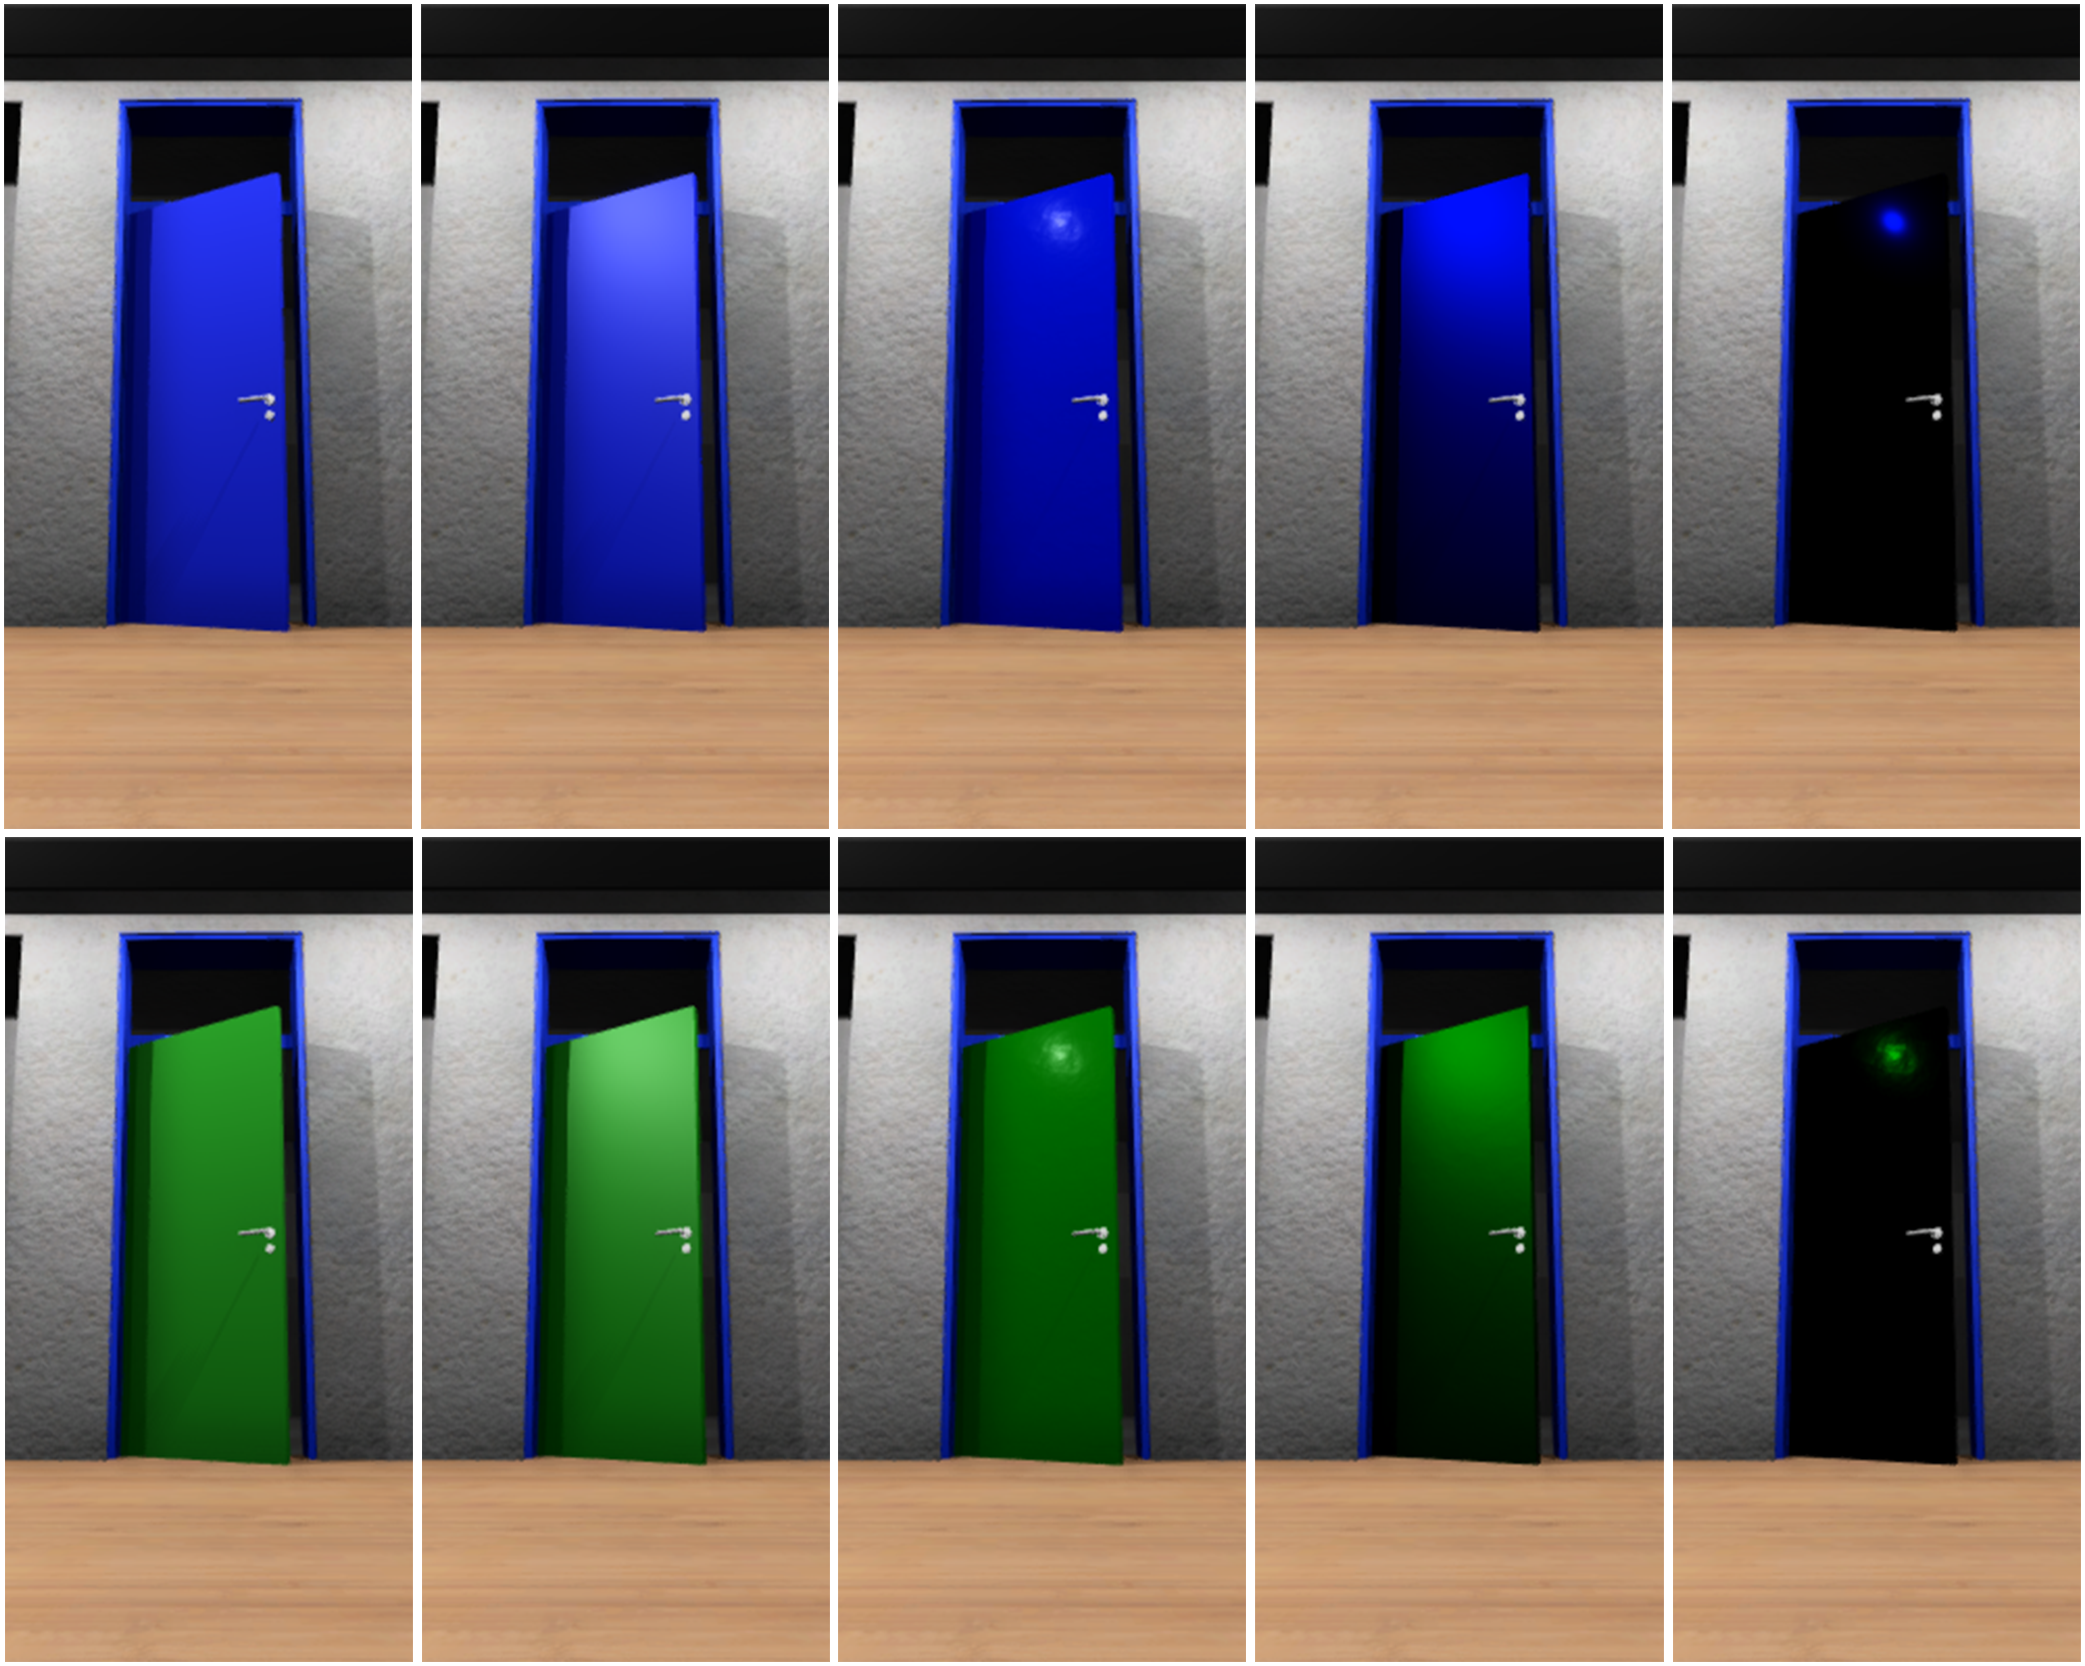
\includegraphics[width=10cm]{tex/img/ch05/Results_Door.png}
\captionof{figure}[Mutators applied to a door]{A door that shows mutated opening angle, color, light-reflection, normal-map and smoothness}
\label{fig:mutated-door}
\end{center}
Similar mutators were implemented for ceiling lights (altering the intensity and range of lights), ambient light (mutating intensity and color) and the sun (altering color, intensity and orientation).

%////////////////////////////////////////////////
\section{Identifying Classifiers}
Proper identification of objects in captured images proved to be a non-trivial problem and the solution to this problem used in \ac{VERE} took multiple approaches until a satisfying solution was found.\\
In order to specify which objects were of interest and shall be identified in captured images, a "Taggable"-component, that had a "Label Name"-attribute that would be treated as a classifier, was implemented and added each relevant object in a scene. The next sections will present the working principles of selected approaches that were implemented and tested and their qualities and drawbacks.

\subsection{Approach I: Using Projection and Raycasting}
The first approach to identifying which objects were visible from a given camera's perspective was to try to cast rays to each "tagged" object and, if hit, project its position from world space into the screen space of the camera. If an object was not hit, it would be occluded by other objects, if the projection from world- to screen space could not be made, the object would not be in the camera's field-of-view and thus not be visible. Cameras in the Unity Engine provide the \emph{"WorldToScreenPoint"} \cite{UnityDocsCamera} method that performs the projection from world space to screen space.\\
Objects in the Unity Engine have transforms that specify location, rotation and scale. These do not translate to colliders of objects though and can not directly be used to determine if an object is hit by a raycast or not as an object may have no colliders that cover its origin: for instance a tire may have its origin at its center so a ray-cast to its origin would not necessarily hit any of its colliders. Therefore, the projection approach needed to consider objects' colliders. A solution to this was to define a set of points to test for along the edges and on the surfaces of colliders: an algorithm would create a point for each vertex of a collider and add a configurable amount of points along edges and surfaces. Each point of these sets could then be tested for using raycasting and projection.\\
Figure \ref{fig:w2s-labelling} shows a door that had these points added to its collider (for a single face) as boxes that were grey and would turn red if proven to be visible by raycasting and projection. Additionally, a red rectangle indicated a region that spanned across all detected points. As can be seen in \ref{fig:labelling01}, \ref{fig:labelling02} and \ref{fig:labelling05} this approach worked reliably in cases where the door took up enough screen space to show multiple points horizontally. In cases where only few points were visible horizontally, as seen in \ref{fig:labelling04}, the indicated region became very thin and in some cases was only one pixel wide, even though parts of the geometry that were not covered by the indicated region were in fact visible. Figures \ref{fig:labelling05}, \ref{fig:labelling06} and \ref{fig:labelling04} were captured while increasing the distance between the camera and the door. These images illustrate a quality of this approach: as long as objects are not fully occluded, parts of them may still be visible from great distance. Due to the decrease in detail in images with the increase of distance from the camera to objects, this may not be usable for training object-recognition software though: distant objects may accommodate for few, if any, pixels in an image and thus be nearly indistinguishable other objects or become hard to identify. This could be solved by limiting the range of rays.\\
A great problem with this approach proved to be its implications on performance: for each object, all of its points needed to be ray-casted for and, if not occluded, projected to the screen. The time it took to test for all objects in a scene was depending on the total amount of objects in a scene, thus the more detailed and larger a scene became, the more time was required to test which objects were visible.\\
\begin{figure}[htp]
    % preliminary
    \sbox\twosubbox{%
      \resizebox{14cm}{!}{%
        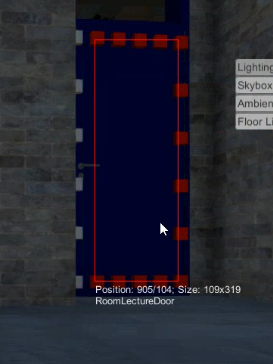
\includegraphics[height=6cm]{tex/img/ch05/Labelling_W2S01a.png}%
        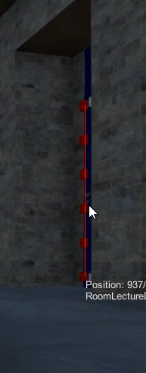
\includegraphics[height=6cm]{tex/img/ch05/Labelling_W2S02a.png}%
        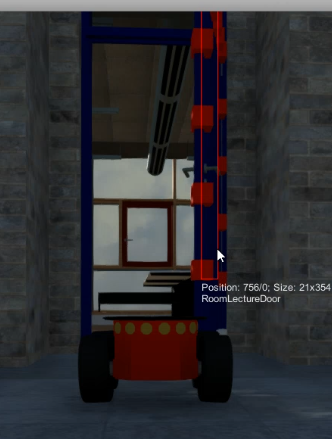
\includegraphics[height=6cm]{tex/img/ch05/Labelling_W2S03.png}%
        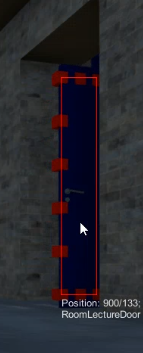
\includegraphics[height=6cm]{tex/img/ch05/Labelling_W2S04a.png}%
        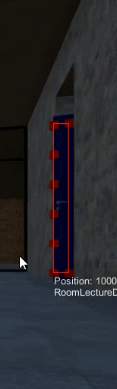
\includegraphics[height=6cm]{tex/img/ch05/Labelling_W2S05a.png}%
        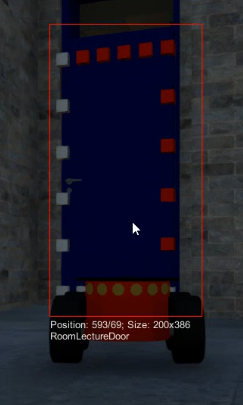
\includegraphics[height=6cm]{tex/img/ch05/Labelling_W2S06.png}%
        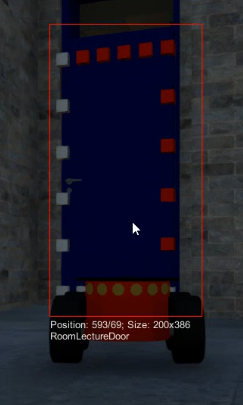
\includegraphics[height=6cm]{tex/img/ch05/Labelling_W2S06.png}%
      }%
    }
    \setlength{\twosubht}{\ht\twosubbox}
    % typeset
    \centering
    \subcaptionbox{\label{fig:labelling01}}{%
      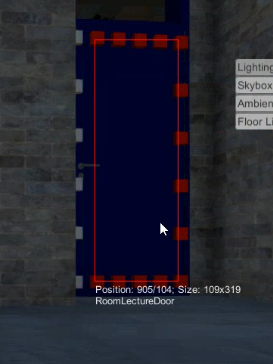
\includegraphics[height=\twosubht]{tex/img/ch05/Labelling_W2S01a.png}%
    }\quad
    \subcaptionbox{\label{fig:labelling02}}{%
      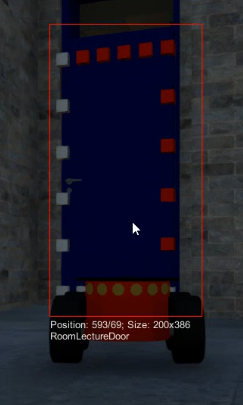
\includegraphics[height=\twosubht]{tex/img/ch05/Labelling_W2S06.png}%
    }\quad
    \subcaptionbox{\label{fig:labelling03}}{%
      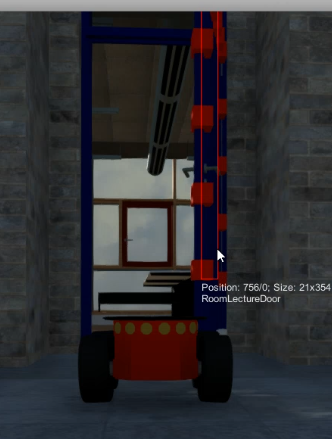
\includegraphics[height=\twosubht]{tex/img/ch05/Labelling_W2S03.png}%
    }\quad
    \subcaptionbox{\label{fig:labelling05}}{%
      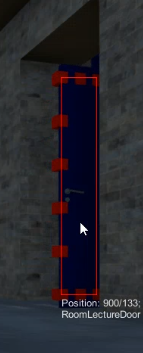
\includegraphics[height=\twosubht]{tex/img/ch05/Labelling_W2S04a.png}%
    }\quad
    \subcaptionbox{\label{fig:labelling06}}{%
      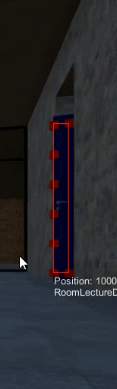
\includegraphics[height=\twosubht]{tex/img/ch05/Labelling_W2S05a.png}%
    }\quad
    \subcaptionbox{\label{fig:labelling04}}{%
      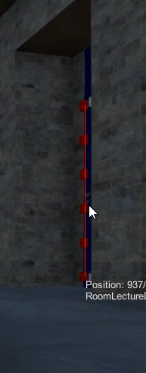
\includegraphics[height=\twosubht]{tex/img/ch05/Labelling_W2S02a.png}%
    }
    \caption[Raycasting and projection approach]{Drawing regions of the identified door from multiple perspectives}
    \label{fig:w2s-labelling}
\end{figure}

Another problem was determining how to create the points on colliders to test for: complex colliders, such as mesh-colliders, could have any shape and any distance from one vertex to another. Those could also have shapes that have vertices that may be occluded by faces and thus never or just rarely be visible, such as convex shapes. As a result, testing for them potentially wasted valuable computing time. Even simple shapes such as cubes and cylinders were not trivial to test for as with increasing scale of objects, the distance between vertices may grow too large to test for: for instance a cube that had an edge length of one meter and had points added to its vertices, three points on each edge and four points evenly distributed on each face, the distance between any neighbouring points would be 25 centimeters. Scaling the cube by a factor of 100 would also scale the distance between said points by 100 and result in neighbouring points being 25 meters away from each other.\\
Solving this problem would require dynamically generating points on colliders, taking the shape and scale of an object into account.

% ** Raycasting
\subsection{Approach II: Casting Rays from screen space}
After using raycasting on every object in the first approach raised performance-concerns, an alternative solution needed to be found. Ideally, a second approach should take the same time to test for visible objects on screen each time it was run and not be influenced by the total amount of objects in a scene.\\
The second approach to identifying objects on images aimed to imitate how humans would process captured images: humans would actually exclusively look at the images presented to them as no other information would be available to them. They may not know about all the other objects in a scene that are not visible in an image and they would most likely not recognize distant objects in images very well due to how few pixels would accommodate for them.\\
Therefore the algorithm implemented in this approach (shown in algorithm \ref{algo:raycasting-screenspace}) scanned the scene from the active camera's perspective in a grid-like fashion. It would use the camera an image was taken with, the \emph{scan-resolution} that defined how many rays it would cast horizontally and vertically and the screen-resolution in pixels and then cast rays that originated from the camera's origin and went through points in screen space, going from top to bottom and left to right (shown in Figure \ref{fig:rclabelling02}). If a cast hit a collider [of a tagged object] it would check whether the same object was already hit before and retrieve a rectangle associated with the object, or create a new rectangle for the object. This rectangle would be extended so that it would contain the screen-coordinate that was used to cast the ray. Once the algorithm finished casting rays it would return a map with rectangles describing regions on screen covered by a single object each associated with their corresponding object (seen in Figure \ref{fig:rclabelling05}). By defining a threshold of the minimum size rectangles needed to be, too small rectangle were discarded, allowing to effectively skip objects that were either too far away from the camera or occluded.\\
\begin{figure}[htp]
    % preliminary
    \sbox\twosubbox{%
      \resizebox{14cm}{!}{%
        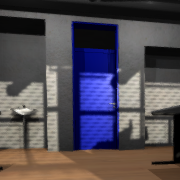
\includegraphics[height=3cm]{tex/img/ch05/RaycastingAlgorithm01.png}%
        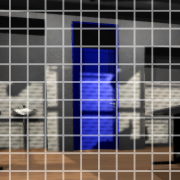
\includegraphics[height=3cm]{tex/img/ch05/RaycastingAlgorithm02.png}%
        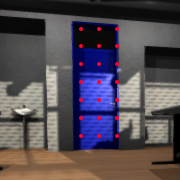
\includegraphics[height=3cm]{tex/img/ch05/RaycastingAlgorithm03.png}%
        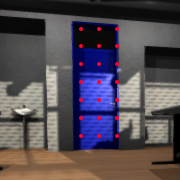
\includegraphics[height=3cm]{tex/img/ch05/RaycastingAlgorithm03.png}%
        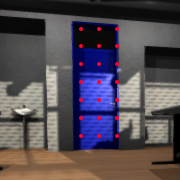
\includegraphics[height=3cm]{tex/img/ch05/RaycastingAlgorithm03.png}%
      }%
    }
    \setlength{\twosubht}{\ht\twosubbox}
    % typeset
    \centering
    %\subcaptionbox{\label{fig:rclabelling01}}{%
    %  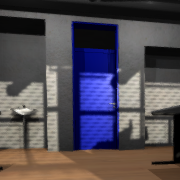
\includegraphics[height=\twosubht]{tex/img/ch05/RaycastingAlgorithm01.png}%
    %}\quad
    \subcaptionbox{\label{fig:rclabelling02}}{%
      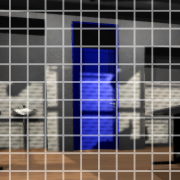
\includegraphics[height=\twosubht]{tex/img/ch05/RaycastingAlgorithm02.png}%
    }\quad
    \subcaptionbox{\label{fig:rclabelling03}}{%
      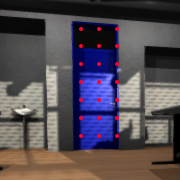
\includegraphics[height=\twosubht]{tex/img/ch05/RaycastingAlgorithm03.png}%
    }\quad%\\
    \subcaptionbox{\label{fig:rclabelling05}}{%
      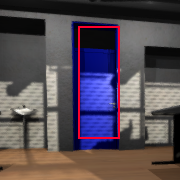
\includegraphics[height=\twosubht]{tex/img/ch05/RaycastingAlgorithm04.png}%
    }\quad
    \subcaptionbox{\label{fig:rclabelling06}}{%
      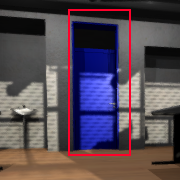
\includegraphics[height=\twosubht]{tex/img/ch05/RaycastingAlgorithm05.png}%
    }
    \caption{Various stages the raycasting algorithm went through}
    %\caption{Ray-Casting algorithm: division of the original image (\ref{fig:rclabelling01}) by horizontal and vertical lines (\ref{fig:rclabelling02}), detection of objects hit by rays (\ref{fig:rclabelling03}), calculating rectangles that cover objects (\ref{fig:rclabelling05}) and extending them to include neighboured area (\ref{fig:rclabelling06})}
    \label{fig:rc-labelling}
\end{figure}


In practice, these rectangles usually would not fully cover objects which is why in the implementation of the algorithm, an option was added to extend the width and height of the rectangles by an adjustable factor, resulting in rectangles that fully covered objects and even included neighbouring area (like parts of the ceiling, wall and floor in Figure \ref{fig:rclabelling06}). Including neighbouring areas in these rectangles adds context to the found objects that may contribute to the quality of detection of object-recognition software. For doors, in this implementation this factor was set to $1.5 \times 1.3$ for width and height, respectively, to accommodate for the distinctive shape of doors.\\
The scan-resolution effectively determines the level of detail that should be detected at which distance and the position of its rays depend on the horizontal and vertical field of view of the camera that is used. The vertical and horizontal field of view of a given camera can be calculated using the focal-length $f$ and sensor-size $d$ (provided by Unity's \emph{physical camera} feature) and the general formula for calculating the angle of view \cite{WikipediaAngleOfView}:
\begin{equation}\alpha = 2 \arctan(\frac{d}{2f})\end{equation}
Unity's camera will have a $36mm \times 24mm$ sensor-size and $20.78mm$ focal-length by default, resulting in a field of view of $82 \times 60$ degrees horizontally and vertically. The maximum distance between two rays being one meter from the camera can be determined by calculating the distance $m$ between any unit-vector (e.g. $v_f = (0, 0, 1)^T$) and the same vector with a rotation along the $y$ and $x$ axis by the scan-resolution $r$ applied to it:\\
\begin{equation}
    \begin{split}
        \alpha & = \frac{x_f}{x_r}, \beta = \frac{y_f}{y_r}\\
        v_r & = \begin{pmatrix}\cos(\alpha) & 0 & -\sin(\alpha) \\ 0 & 1 & 0 \\ \sin(\alpha) & 0 & \cos(\alpha)\end{pmatrix} \times
        \begin{pmatrix}1 & 0 & 0 \\ 0 & \cos(\beta) & \sin(\beta) \\ 0 & -\sin(\beta) & \cos(\beta)\end{pmatrix} \times
        \begin{pmatrix}0 \\ 0 \\ 1\end{pmatrix}\\
            & = \begin{pmatrix}(-\sin(\alpha)) \cos(\beta) \\ \sin(\beta) \\ \cos(\alpha)\end{pmatrix}\\
        m   &= || v_f - v_r || = \sqrt{(\sin(\alpha) (-\cos(\beta)))^2 + \sin(\beta)^2 + \cos(\alpha)^2}
    \end{split}
\end{equation}

Using a rather rough scan-resolution of $10 \times 5$, at any distance of $n$ meters from the camera, neighbouring rays would be at most $0.866 \times n$ meters away from each other. Such rough scan-resolutions may be used to identify large objects in images and skip smaller ones.\\
The execution-time this algorithm needed to identify objects in images was not depending on the number of tagged objects in the scene anymore but instead depended on the time needed to perform a fixed set of ray-casts. This allowed scenes to grow in size and complexity as the number of tagged objects would not influence the labelling-process anymore. In order to run this algorithm in real-time, a maximum distance had to be defined so that casting individual rays was deterministic. Depending on the scenario at hand, this limit should be set to the highest distance the object-recognition should still be able to detect objects at. Also, by defining appropriate scan-resolutions, the resulting regions would not include objects that were too far away from the camera or only had small parts of them visible.

\section{Generating Datasets}
Right after loading a scene \ac{VERE} created a list of all distinct labels associated to tagged objects. When it saved captured images it created a JSON file that included information about the position and rotation of the camera that was used to capture the image and a list of identified objects along with the position and size (in pixels) of their associated region in the image and their label. It also saved a textfile for each image that can be used with the neural network framework \emph{"Darknet"}.\\
In order to shorten the duration of the recording process, identification of objects in the scene was only performed once per mutation cycle as the robot did not move during the capture process. However this optimization did not take mutators into account that altered the geometry or transforms of objects, potentially leading to inaccurate detection regions.

\subsection{Inspecting the Generated Output}
To verify the correctness of the output generated by \ac{VERE} an application was needed that parsed the generated files and visualized the regions of identified objects. A desktop application was implemented under the working title \emph{VERE-Viewer}. It used utilized components provided by the .NET Framework for its UI.

\begin{center}
\noindent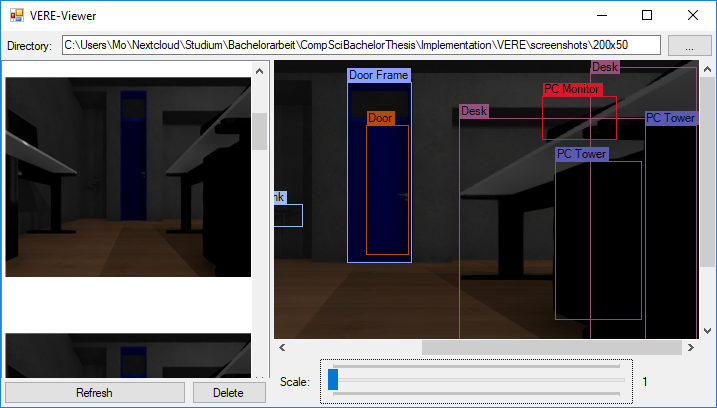
\includegraphics[width=14cm]{tex/img/ch05/VERE_Viewer_Application02.png}
\captionof{figure}[The VERE-Viewer application]{VERE-Viewer visualizing regions of identified objects}
\label{fig:vere-viewer}
\end{center}

%////////////////////////////////////////////////
\section{Performance of the Software}
There were several factors that had an impact on \ac{VERE}'s performance. Aside from the configurable parameters (scan resolution and screen or image resolution), the hardware \ac{VERE} would run on limited its performance. Contrary to regular games it did not only render frames to screen but captured an image each frame and saved it along with meta data. Rendering frames utilized the GPU while casting rays to identify objects was performed on the CPU. Lastly, saving the records to disk required a drive that handled writing multiple files in short intervals well.\\
To test \ac{VERE} it was run on a machine with a \textit{Intel i5-2310} CPU, \textit{NVIDIA GeForce GTX 760} GPU and a \textit{Kingston A400} SSD.
Table \ref{table:vere-performance} shows how \ac{VERE} performed on this hardware in automatic mode (shown in detail in section \ref{ch04-control-flow}), completing three mutation-cycles with images using a very low resolution ($640 \times 360$ pixels), a common resolution used in modern monitors ($1920 \times 1080$ pixels, commonly referred to as \textit{"Full HD"} and \textit{"1080p"}) and a very high resolution that is used in modern high end displays (also known as \textit{"4K UHD"} and \textit{"4K"}). The scan resolution chosen was $200 \times 50$.

\begin{table}[htbp]
    \centering
    \begin{tabular}{c|c|c|c|c|c|c}
        \hline
              \thead{Image\\Resolution} & \thead{Cycle \#1 (s)} & \thead{Cycle \#2 (s)} & \thead{Cycle \#3 (s)} & \thead{Cycle\\Average (s)} & \thead{Captures \textbackslash s} \\
        \hline
            $640 \times 360$ & 49.64 & 53.97 & 51.41 & 51.67 & 18.79 \\
            $1920 \times 1080$ & 260.32 & 272.01 & 287.14 & 273.16 & 3.55 \\
            $3840 \times 2160$ & 871.69 & 903.18 & 899.74 & 891.54 & 1.09 \\
    \end{tabular}
    \caption[Comparison of recording sessions]{Comparison of recording sessions with different image resolutions}
    \label{table:vere-performance}
\end{table}